\documentclass[10pt, a4paper]{article}

\usepackage{amsmath}
\usepackage{amssymb}
\usepackage{graphicx}
\usepackage{listings}
\usepackage{color}
\usepackage[section]{placeins}
\usepackage{paralist}

\usepackage{caption}
\usepackage{subcaption}

\definecolor{mygreen}{rgb}{0,0.6,0}
\definecolor{mygray}{rgb}{0.5,0.5,0.5}
\definecolor{mymauve}{rgb}{0.58,0,0.82}

\lstset{ %
  backgroundcolor=\color{white},
  basicstyle=\footnotesize,
  breakatwhitespace=false,
  breaklines=true,
  captionpos=b,
  commentstyle=\color{mygreen},
  escapeinside={\%*}{*)},
  extendedchars=true,
  keepspaces=true,
  keywordstyle=\color{blue},
  rulecolor=\color{black},
  showspaces=false,
  showstringspaces=false,
  showtabs=false,
  stepnumber=2,
  stringstyle=\color{mymauve},
  tabsize=2,
}

\hyphenation{GENITOR}

\newcommand*{\titleGM}{\begingroup
\hbox{ 
\hspace*{0.2\textwidth} 
\rule{1pt}{\textheight} 
\hspace*{0.05\textwidth} 
\parbox[b]{0.75\textwidth}{ 

{\noindent\Huge\bfseries Solving Travelling Salesman Problems using Genetic
 Algorithms}\\[2\baselineskip] % Title
{\large \textit{SEM6120 - Assignment 2}}\\[4\baselineskip] % Tagline or further description
{\Large \textsc{Alexander D Brown (adb9)}} % Author name

\vspace{0.5\textheight} 
}}
\endgroup}


\title{Genetic Algorithms}
\author{Alexander D Brown (adb9)}

\begin{document}
\titleGM 
\tableofcontents
\newpage

\section{Introduction}
This report investigates the use of Genetic Algorithms to solve the Travelling
Salesman Problem, introducing both topics as well as previous research and 
techniques.

Following this the design for the solution implemented will be detailed,
focusing from high level system design to annotated code section to explain the
choice behind the implementation.

This implementation is then used to produced the results in
section~\ref{sec:results} which give an insight into the affects of different
crossover and mutation schemes on the performance of the genetic algorithm,
specifically looking at crossover operators, crossover rate and mutation rate.


\subsection{Genetic Algorithms}
Genetic algorithms are a biologically-inspired approach to heuristic search 
that mimic natural selection. Unlike many other evolutionary strategies and
evolutionary programming, they are not designed to solve a specific problem,
but are designed to solve the problem of optimisation which is made difficult
by substantial complexity and uncertainty\cite{Holland1992Adaptation}.

\subsection{Travelling Salesman Problem}
The Travelling Salesman Problem is a well-known NP-hard optimisation problem
which asks the question: \textit{``Given a number of cities and the distances 
between these cities, find the shortest touch which visits each city exactly 
once and returns to the first city.''}

Assuming each city is connected to every other city, this problem reaches a
complexity of $O(n!)$ and is very resource intensive to brute force a problem
with any decent number of nodes quickly become too larger problem to solve
within a reasonable amount of time.

There are many heuristic algorithms which have been applied successfully to the
Travelling Salesman Problem, including both Evolutionary and Genetic 
Algorithms.

Though the nature of Genetic Algorithms are suited to the optimisation of a
Travelling Salesman Problem, normal methods of crossover and mutation cannot,
generally, be applied directly to the problem. The representation of 
chromosomes has to be ordered (i.e.\ each city must appear once and only once)
and additional methods of crossover and mutation have had to be designed for
these ordered chromosomes.

\newpage
\section{Design}
This section describes the design of the implementation, from high-level
concepts like the system design, to details on the implementation and uses of
programming paradigms to make the code succinct.

\subsection{System Design}
% Overall idea: modularise system
As with most coding problems with multiple options, a modular approach is
necessary to keep code quality high. This is typically done by defining
high-level interfaces for the changeable elements. In this case the obvious
three interfaces are:

%  - Define high-level classes for selection, crossover & mutation
\begin{enumerate}
\item Selection Scheme
\item Crossover Scheme
\item Mutation Scheme
\end{enumerate}

From these high-level classes, concrete sub-classes can be written to perform
the actual logic. An example of this would be a specific class for Order-1
based crossover.

%  - Use factories to generate specific classes based of input
This leaves the problem of how to accesses these classes based on an input
string; the easiest method for this is to use factories to access these 
classes, cutting down the number of specific imports required and centralising
the logic for creating them.

%  - Discuss the structure of graphs and ways to cut down the amount of memory
%    used.


\subsubsection{Language Choice}
Python was the choice of language, it is a dynamically typed language which 
provides several programming paradigms to work with, including procedural,
object-orientated and functional paradigms.

It is a language the author is very familiar with and has the advantage of
having many open source libraries to perform different scientific functions;
some of these libraries have been used in the course of this project, including
the popular \texttt{numpy} library for number processing and 
\texttt{matplotlib} to produce graphs.

The strange choice of \texttt{pygame} was made for the choice of displaying the
GUI, but this games library gives simple yet powerful access to OpenGL and also
manages platform dependencies.

\subsubsection{UML Class Diagram}

Figure~\ref{fig:uml} shows the initial UML Class diagram for this project.
There are some elements which break from typical object-orientated design,
noticeably the representation of nodes in a graph as a map of integers to a
turple of float, these parts are done so to re-use internal data structures of
the Python programming language to speed up the implementation of many 
features.

\begin{figure}[h]
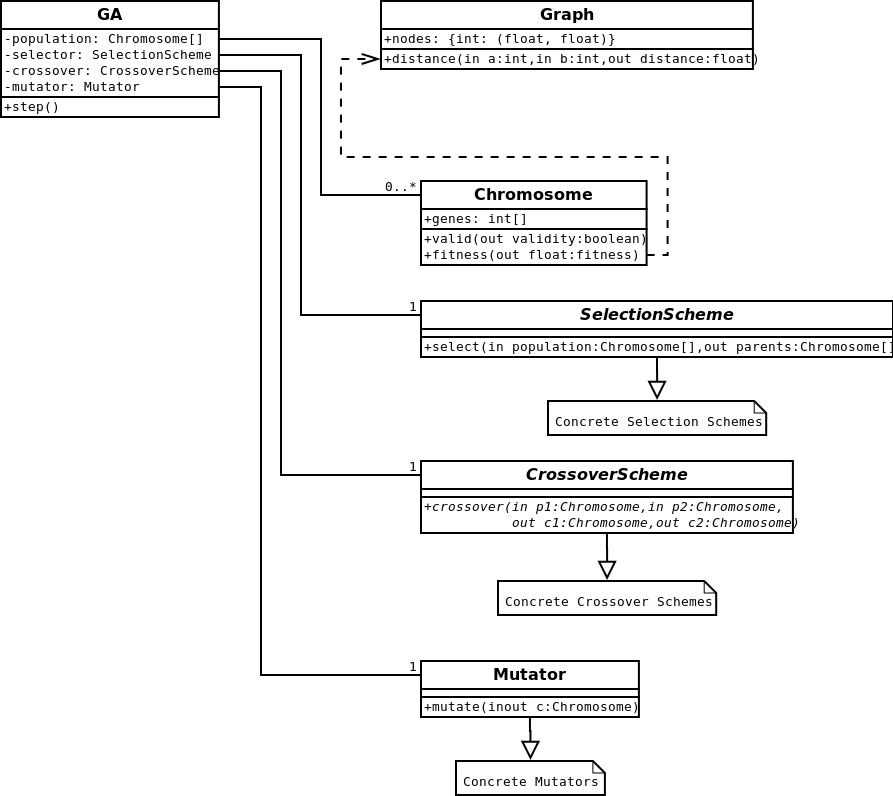
\includegraphics[width=\textwidth]{img/uml.png}
\caption{UML Class Diagram for the Genetic Algorithm}
\label{fig:uml}
\end{figure}

This design is such that factories exist to create selection schemes, crossover
schemes and mutators based on an input string to facilitate the switching of
these elements via command line arguments.

This design was slowly improved through the project; the
\texttt{CrossoverScheme} class implemented the \texttt{crossover} method, 
which then called a separate method, \texttt{do\_crossover}, to generate 
\texttt{c1} based on \texttt{do\_crossover(p1, p2)} and \texttt{c2} on 
\texttt{do\_crossover(p2, p1)} to make the processing more uniform. Subclasses
were still able to override the \texttt{crossover} method, but were encouraged
to implement a \texttt{do\_crossover} method unless the scheme required a
different behaviour of child generation.


\subsubsection{Representation of Graphs}

The actual of representation of a graph is a map of the node identifier to the
$x$ and $y$ co-ordinates of that node (as a tuple). This allows easy look up 
of nodes within the map to get the position of the node. This was chosen 
because of the representation of the problem in chromosomes - each gene 
represents a node in the graph.

With this representation, the fitness function would be the distance of the 
tour represented by these nodes:

\begin{equation}
d_{tour} = \sum^{N}_{i=0}{
  \begin{cases}
    d(n_i, n_{i+1}) & \text{if } i+n < N \\ 
    d(n_i, n_0)     & \text{else}
  \end{cases}
}
\end{equation}

Programatically, with the advantage of the functional and in-built elements of 
Python, this can be simplified to:

\lstset{language=Python}
\begin{lstlisting}[language=Python, caption=Distance of a tour]
def d_tour():
  # Move the first element of the array to the end.
  shifted = nodes[1:] + nodes[:1]
  return sum([distance(i, j) for (i, j) in zip(nodes, shifted)])
\end{lstlisting}

\subsection{Use of Functional Programming Paradigms}

As Python implements several different programming paradigms a lot of problems
can be solved with a different approach than other languages can. Both genetic
algorithms and the travelling salesman problem lend themselves towards a more
functional approach with a lot of list processing. Using Pythons list
comprehensions and the in-built list functions shortened the amount of code 
required and makes the code a lot easier to understand for those who are used 
to this approach.

A very good example of this is the method for evaluating chromosomes in a
population, returning a list sorted from the best to the worst:

\begin{lstlisting}[language=Python, 
                   caption=Using function elements to improve sustinctness and
                           readability]
def eval(population):
  return sorted(population, 
                key = lambda chromosome: chromosome.fitness())
\end{lstlisting}


\subsection{Crossover Strategies}

Three main types of crossover strategies were implemented for this research:

\begin{enumerate}
\item Cycle Crossover,
\item Order Crossover Operator,
\item M-Crossover Operator.
\end{enumerate}

All three are designed to work with ordered chromosomes, meaning they can be
applied directly to the Travelling Salesman Problem without any modification.

\subsubsection{Cycle Crossover}

Cycle crossover is one of the simplest order-based crossover operators. Unlike
many other forms of order-based operators it make no effort to preserve parts 
of the parent chromosomes.

To produce a child, $c$, from parents $p_1$ and $p_2$ a randomly selected point
$i$ is chosen. The gene at $i$ in $p_1$ ($r = p_1(i)$) is removed and replaced 
with $p_1(i) = p_2(i)$. The position of the removed allele $r$ is found in 
$p_2$ such that $i = index(r, p_2)$. This process is repeated until a cycle
occurs (i.e. the removed allele $r$ is the same as the initially removed 
allele).

Figure~\ref{fig:cycle-crossover} shows this process step by step on two ordered
chromosomes. Note that it only by chance that parts of the tour are preserved.

\begin{figure}[h]
\centering
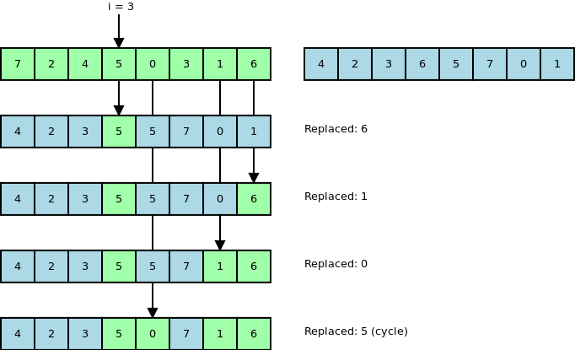
\includegraphics[width=0.8\textwidth]{img/cycle-crossover.png}
\caption{Cycle Crossover}
\label{fig:cycle-crossover}
\end{figure}


\subsubsection{Order Crossover Operator}

The order crossover operator is another simple order-based crossover operator.
Unlike cycle crossover, it preserves at least part of a tour from one of the
parents.

To produce a child, $c$, from parents $p_1, p_2$, a random segment from $p_1$ 
is appended to the remaining genes from $p_2$, omitting any alleles that are
also in the segment from $p_1$.

Figure~\ref{fig:order-crossover-operator} shows this process step by step on
two ordered chromosomes. Note that at least a part of the tour is always
preserved and that it is often the case that a part of a tour from $p_1$ and
$p_2$ is preserved in $c$.

\begin{figure}[h]
\centering
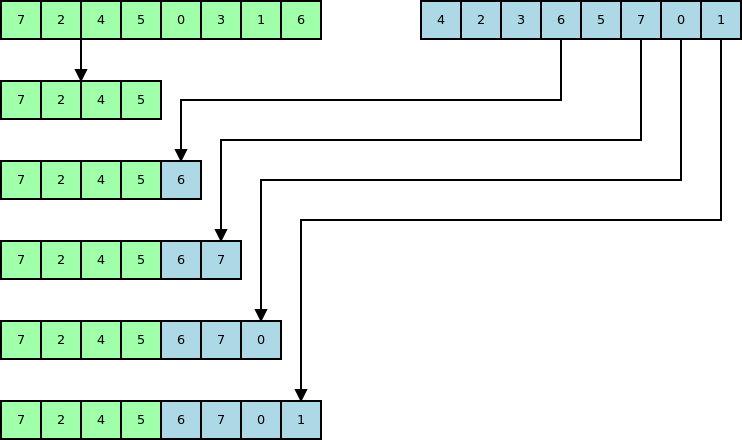
\includegraphics[width=0.8\textwidth]{img/order-crossover-operator}
\caption{Order Crossover Operator}
\label{fig:order-crossover-operator}
\end{figure}


\subsubsection{M-Crossover Operator}

The m-crossover operator\cite{Mudaliar2013Unraveling} produces multiple 
offspring ($C$) from parents $p_1, p_2$ then selects the best two from this 
process.

Like with the order crossover operator, this is based on segmenting the
chromosomes. However, both chromosomes are split into several segments. Every
segment of $p_1$ is inserted at any point in front, behind or between the
segments of $p_2$ and vice versa. The new, elongated chromosome is then
processed such that any allele in the added segment is removed from all other
segments to produce the child at that point.

The fitness of these children is then evaluated and the best two are carried 
forward as the offspring of these parents.

\begin{figure}[h]
\centering
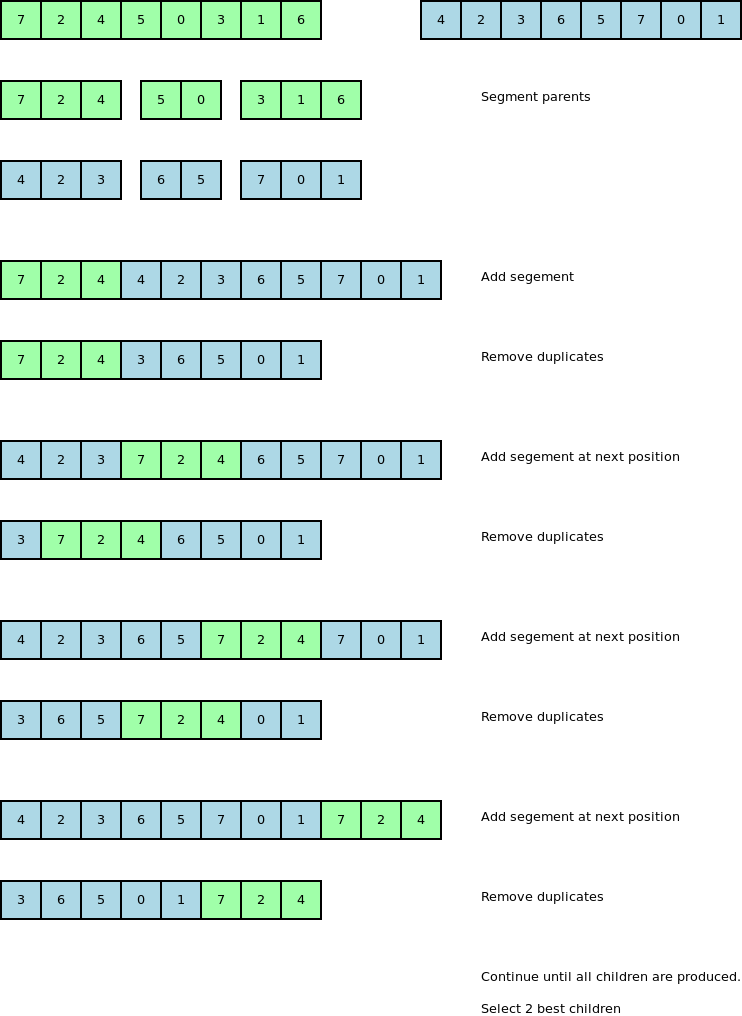
\includegraphics[width=0.8\textwidth]{img/m-crossover-operator}
\caption{M-Crossover Operator}
\label{fig:m-crossover-operator}
\end{figure}


\subsection{Mutation Operators}

Two mutation operators were implemented for this problem. Again, as with
crossover, normal mutation operators cannot be directly applied to a genetic
algorithm with ordered chromosomes.

One fairly standard mutation operators for ordered chromosomes is the swapping
of genes. To do this, two genes are selected at random and are swapped, ensuring
that the chromosome is always still valid.

This mutation operator does have the problem that it can significantly change
tours and though this encourages variety, it may introduce too much.

To help reduce this, a second mutation operator was designed so that only
adjacent genes are swapped. This helps to preserve most of the tour whilst
changing small parts of it.


\subsection{Parallelisation}

Although genetic algorithms benefit greatly from a multi-threaded approach,
there was not enough time to make the code parallel. The attempts made to do so
led to many errors which would have caused major changes in the code (i.e.\
changing from an object-orientated approach to a procedural one) which were too
costly to take.

The author's knowledge of multi-threading in Python is not that great so there
may have been a better solution, but the time was better spent on implementing
other crossover operators for comparison.


 
\newpage
\section{Results}
\label{sec:results}

To gain some insight from the implementation the impacts of several aspects of
the GA were investigated: the crossover strategy, the crossover rate, the
mutation rate and the mutation scheme.

Figure~\ref{fig:ga-running} shows an example of the genetic algorithm in
progress.

\begin{figure}[h]
\begin{subfigure}[b]{0.49\textwidth}
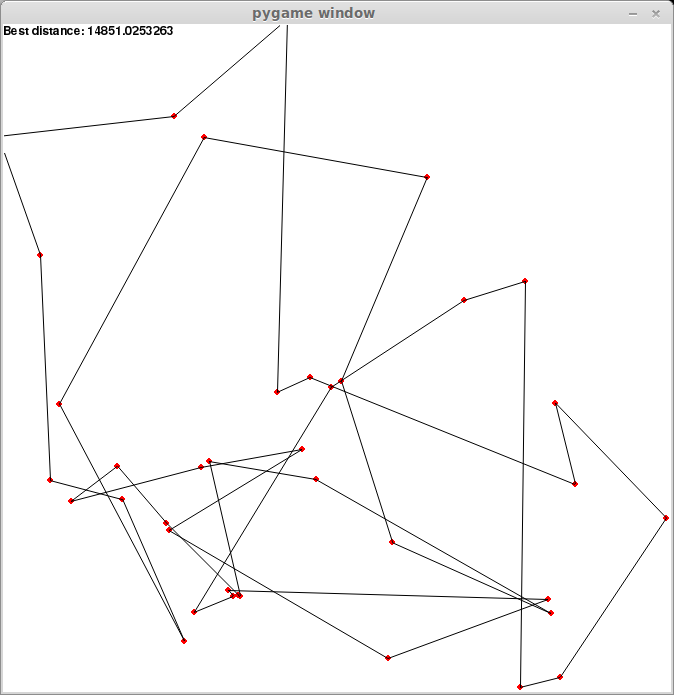
\includegraphics[width=\textwidth]{img/ga-initial}
\caption{At early generation.}
\end{subfigure}
\begin{subfigure}[b]{0.49\textwidth}
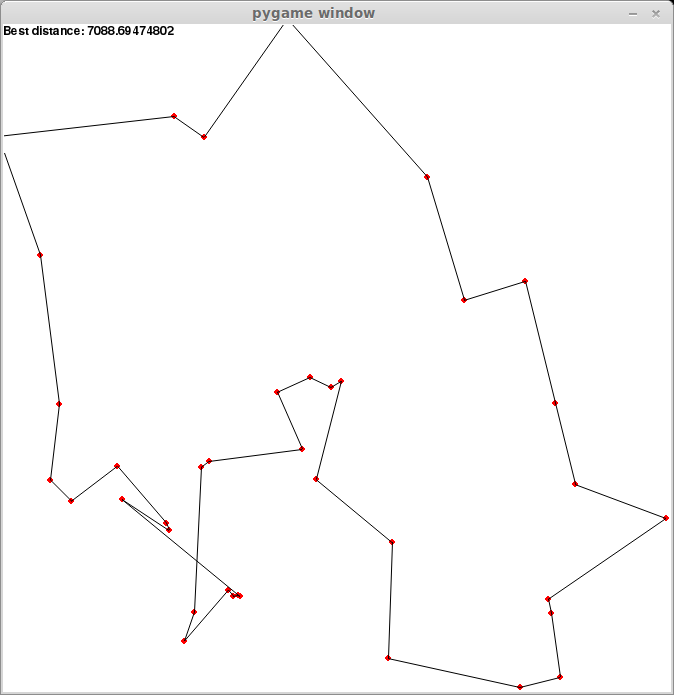
\includegraphics[width=\textwidth]{img/ga-in-progress}
\caption{At a late generation.}
\end{subfigure}
\caption{The Genetic Algorithm at different points in the runtime.}
\label{fig:ga-running}
\end{figure}

\subsection{Impact of Crossover Strategies}
The crossover strategy is one of the biggest influences on the performance of
genetic algorithm, the first set of experiments should focus on the differences
between them.

All results are run over 500 generations and averaged over 100 experimental 
test runs.

Figure~\ref{fig:crossover-results} shows the experimental results for all three
of the crossover operators.

Cycle crossover consistently performs worse than the other two, likely because
it doesn't preserve good parts of tours. It also has very little variation
between individuals of the population as the average fitness is very close to
the best fitness.

It should be noted from the visualisation of the GA that cycle crossover tends
quickly towards a local minima, but has difficulty finding lower minima. It is
likely that with a higher mutation rate cycle crossover would perform better as
more varied possibilities would be considered.

The m-crossover operator performs fairly well but, as with cycle crossover,
converges quickly which slows the rate of performance after a small number of
generations. This is fairly intuitive as it is constantly selecting the best
possible offspring from the parents.

It seems that the m-crossover operator is good for getting a quick estimate of
the problem in a low number of generations. But for finding a solution as close
to the optimal as possible it would seem that it isn't the best crossover
operator.

The other issue with the m-crossover operator is that it consumes a lot more
resources and time than the other two, as it has to generate extra children,
evaluate them and then only choose two of them.

By far the best operator for reaching a solution close to the optimal is the
order crossover operator. It manages to keep plenty of variety in the 
population whilst still managing to get the best fitness very close to the
global minima.

All three operators would be trivial to make parallel (though due to time
constraints the author did not do so) and so could be made more efficient in
term of runtime.

Of the three it feels the order crossover operator is the most useful for
general application, whilst the m-crossover operator would suit a problem which
would a good solution quickly. The cycle crossover is very simple, but should
have a performance similar to the order crossover operator.


\begin{figure}[h]
\centering

\begin{subfigure}[b]{0.67\textwidth}
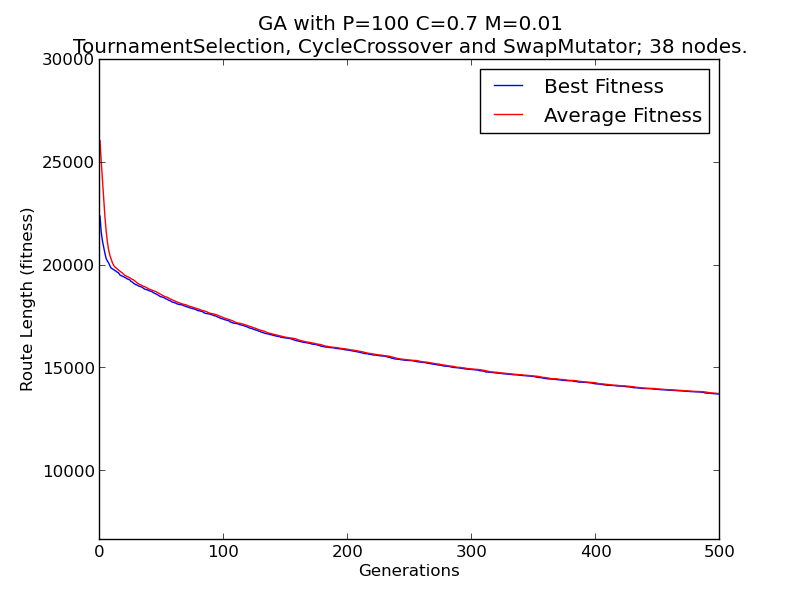
\includegraphics[width=\textwidth]{img/results/cyclecrossover/swapmutator/n38p100c07m001}
\caption{Cycle Crossover}
\end{subfigure}
~
\begin{subfigure}[b]{0.67\textwidth}
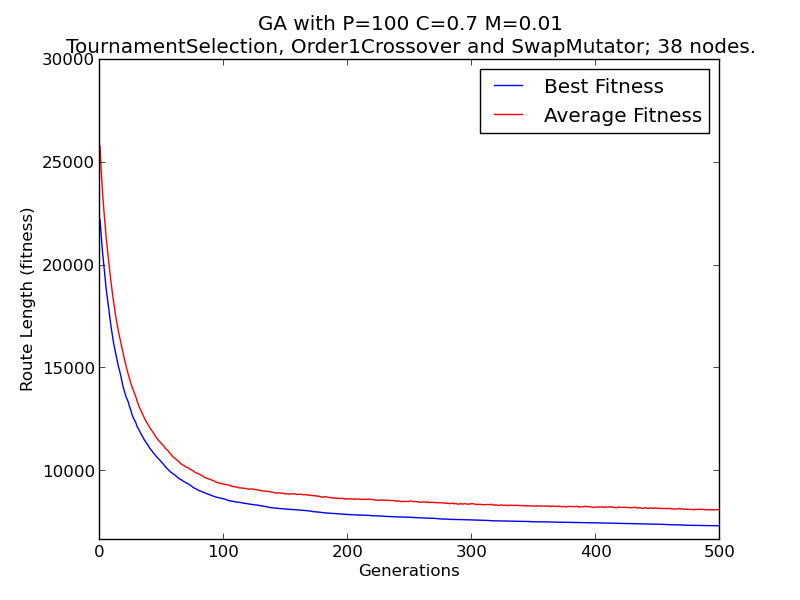
\includegraphics[width=\textwidth]{img/results/order1crossover/swapmutator/n38p100c07m001}
\caption{Order Crossover Operator}
\end{subfigure}
~
\begin{subfigure}[b]{0.67\textwidth}
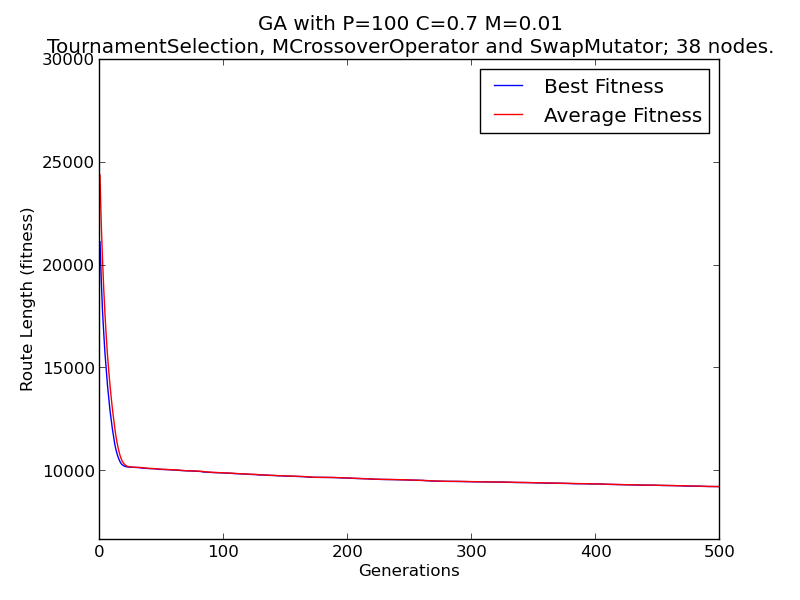
\includegraphics[width=\textwidth]{img/results/mcrossoveroperator/swapmutator/n38p100c07m001}
\caption{M-Crossover Operator}
\end{subfigure}

\caption{Results on different crossover operators on a data set with 38 nodes.
         All used a population of 100, crossover rate of 0.7, mutation rate of 
         0.01 and the swap mutator}
\label{fig:crossover-results}
\end{figure}


\subsection{Impact of Crossover Rate}
The next step was to investigate the impact of crossover rate on the 
performance of a genetic algorithm.

All results are run over 500 generations and averaged over 100 experimental 
test runs using the order crossover operator which was the best of the three
crossover operators chosen.

Figure~\ref{fig:crossover-rate-results} shows the experimental results for with
three different crossover rates: 0.1, a very low crossover rate; 0.7, a 
commonly used crossover rate; and 0.9, a very high crossover rate.

It should be noted that this implementation is such that crossover rate defines
not only the chances of crossover being performed, but also the ratio of the
population which is made up of newly generated offspring. For example, if the
crossover rate is $0.7$ then the offspring will make up $70\%$ of the new
population and the rest will be the best $30\%$ of the old population.

The results show slightly interesting results. The results from the crossover
rate of 0.1 is intuitive, a low crossover rate is expected to elongate the
number of generations it takes to optimise a solution. It also has a profound
affect on the convergence of the population in that it converges quickly, which
appears to be uncommon for the order crossover operator.

Where the results get interesting is that the higher crossover rate of 0.9
reaches a better best solution than the standard crossover rate of 0.7. This 
may be a result of the implementation of crossover rate, or because it works
well with the order crossover operator. However, as the other crossover
operators perform similarly, one could say that it is because of the
implementation of the genetic algorithm.

The other possibility is that a high crossover rate is good for the travelling
salesman problem, however most literature in the area would suggest otherwise.

\begin{figure}[h]
\centering

\begin{subfigure}[b]{0.67\textwidth}
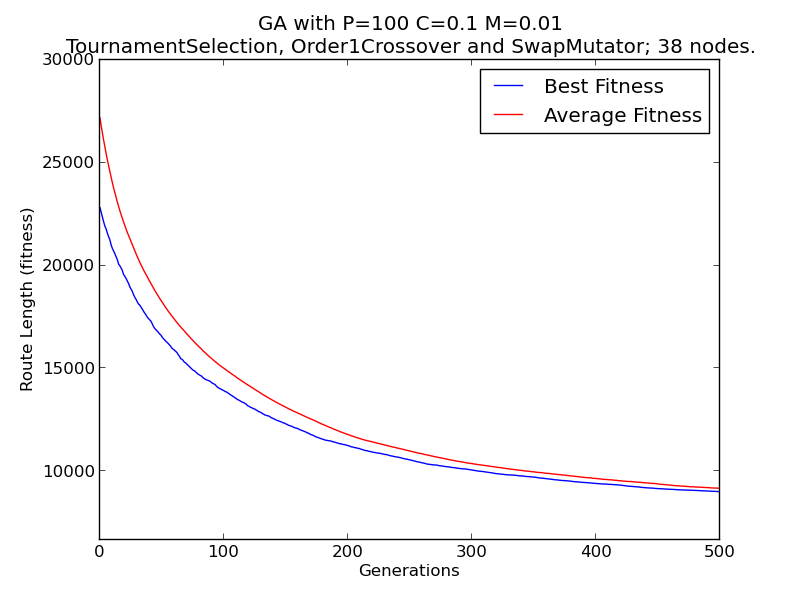
\includegraphics[width=\textwidth]{img/results/order1crossover/swapmutator/n38p100c01m001}
\caption{$c = 0.1$}
\end{subfigure}
~
\begin{subfigure}[b]{0.67\textwidth}
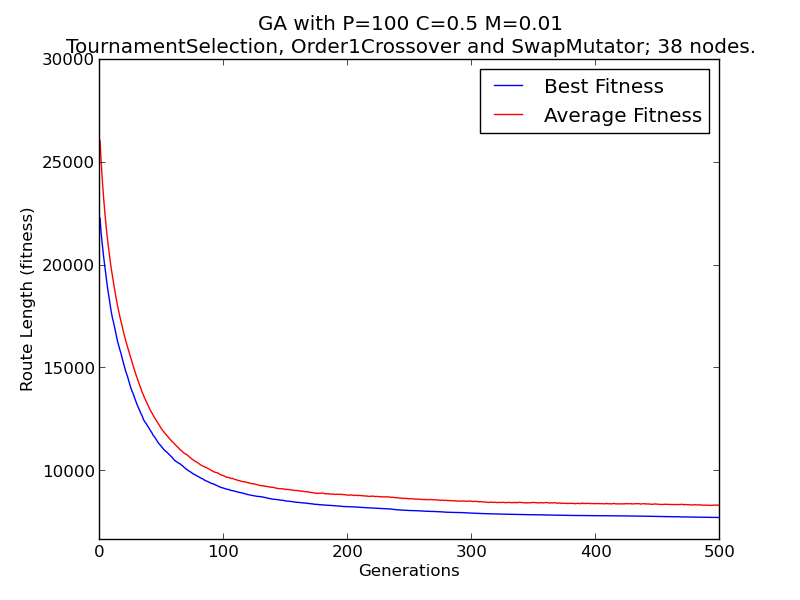
\includegraphics[width=\textwidth]{img/results/order1crossover/swapmutator/n38p100c05m001}
\caption{$c = 0.7$}
\end{subfigure}
~
\begin{subfigure}[b]{0.67\textwidth}
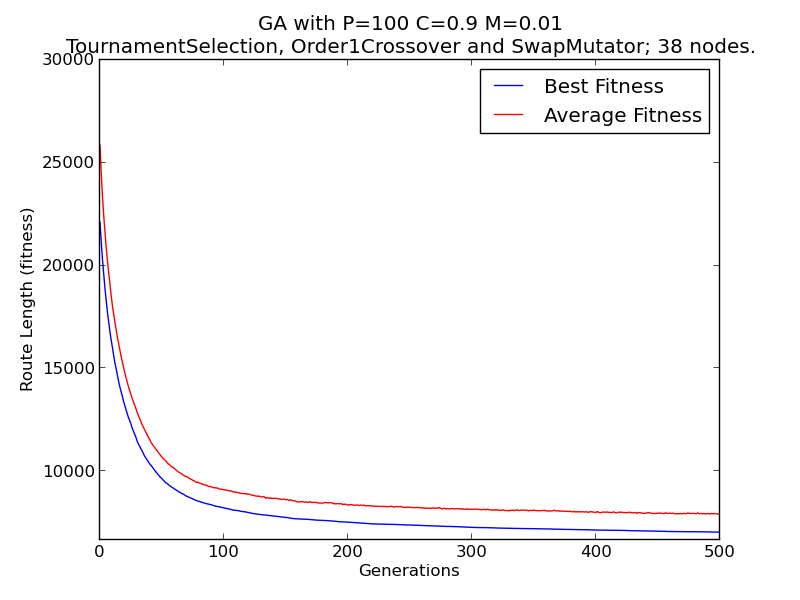
\includegraphics[width=\textwidth]{img/results/order1crossover/swapmutator/n38p100c09m001}
\caption{$c = 0.9$}
\end{subfigure}
\caption{Results on different crossover rate ($c$) on a data set with 38 nodes.
         All used a population of 100, mutation rate of 0.01 with the order
         crossover operator and the swap mutator}
\label{fig:crossover-rate-results}
\end{figure}


\subsection{Impact of Mutation Rate}

All results are run over 500 generations and averaged over 100 experimental 
test runs using the order crossover operator and a crossover rate of 0.7.

Figure~\ref{fig:mutation-rate-results} show the experimental results for three
mutation results: 0.01, a standard mutation rate for small populations; 0.25 a
medium mutation rate; and 0.5, a relatively high mutation rate.

Interestingly the change of mutation rate have very little affect, other than to
increase the variance of the population. For the higher mutation rate it does
the speed of optimisation as well as increasing the variance. However, it is
interesting that the medium mutation rate of 0.25 produces a better result than
the standard mutation rate of 0.01. However as the population size is 100, it is
on the cusp of needing a standard mutation rate of 0.1.

\begin{figure}[h]
\centering

\begin{subfigure}[b]{0.67\textwidth}
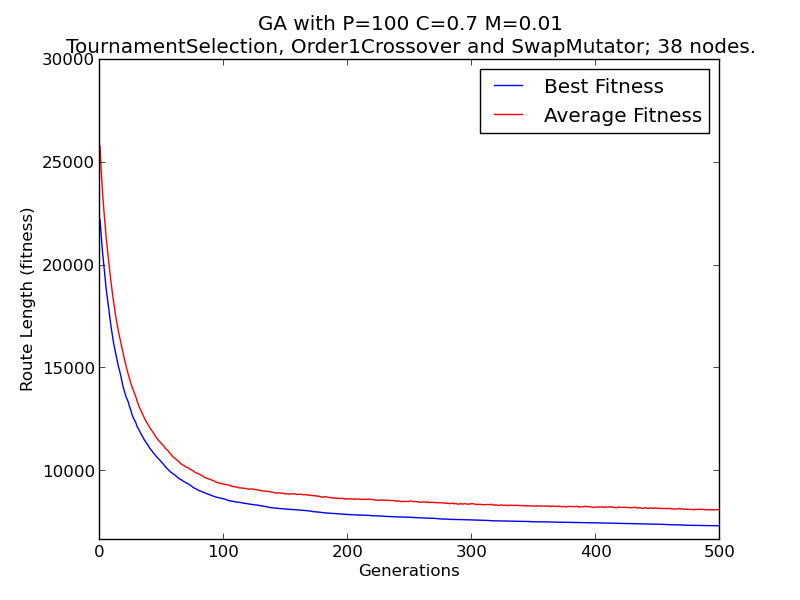
\includegraphics[width=\textwidth]{img/results/order1crossover/swapmutator/n38p100c07m001}
\caption{$m = 0.01$}
\end{subfigure}
~
\begin{subfigure}[b]{0.67\textwidth}
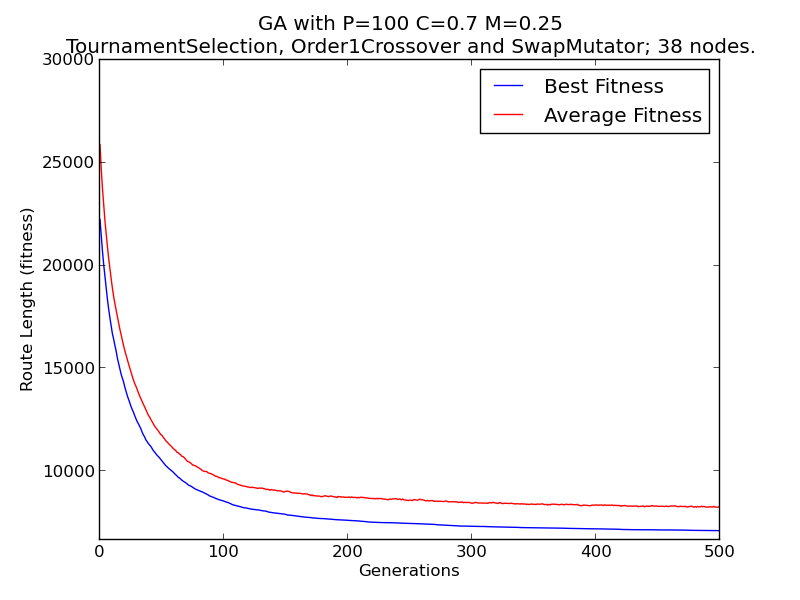
\includegraphics[width=\textwidth]{img/results/order1crossover/swapmutator/n38p100c07m025}
\caption{$m = 0.25$}
\end{subfigure}
~
\begin{subfigure}[b]{0.67\textwidth}
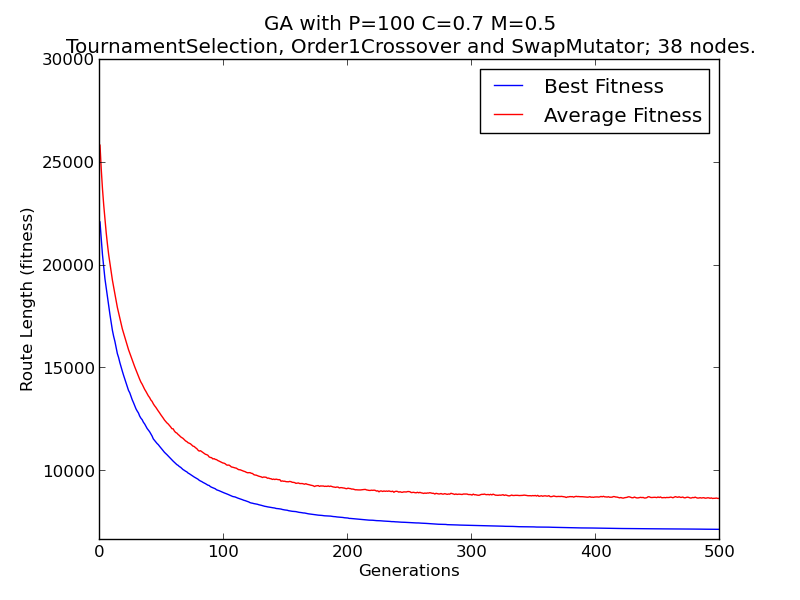
\includegraphics[width=\textwidth]{img/results/order1crossover/swapmutator/n38p100c07m05}
\caption{$m = 0.5$}
\end{subfigure}
\caption{Results on different mutation rate ($m$) on a data set with 38 nodes.
         All used a population of 100, crossover rate of 0.7 with the order
         crossover operator and the swap mutator}
\label{fig:mutation-rate-results}
\end{figure}


\subsection{Impact on Mutation Operator}

All results are run over 500 generations and averaged over 100 experimental 
test runs using the order crossover operator and a crossover rate of 0.7.

Figure~\ref{fig:mutation-results} show the experimental results for the swap
mutator operator and the swap adjacent operator.

As is fairly intuitive, the swap adjacent operator reduces the variety in the
population. However, it doesn't allow the GA to get as close to the optimal
solution as the swap operator does.

Although the swap operator doesn't preserve tours as well, it seems to allow
the genetic algorithm to easier get out of local minima, whilst limiting the
swap to only adjacent genes is too limiting and the algorithm can often get
caught in local minima.

It may be the case that limiting the swap to the two (or more) adjacent nodes
would help it to avoid this problem and this may be an interesting, if small,
piece of research to perform.

\begin{figure}[h]
\centering
\begin{subfigure}[b]{0.67\textwidth}
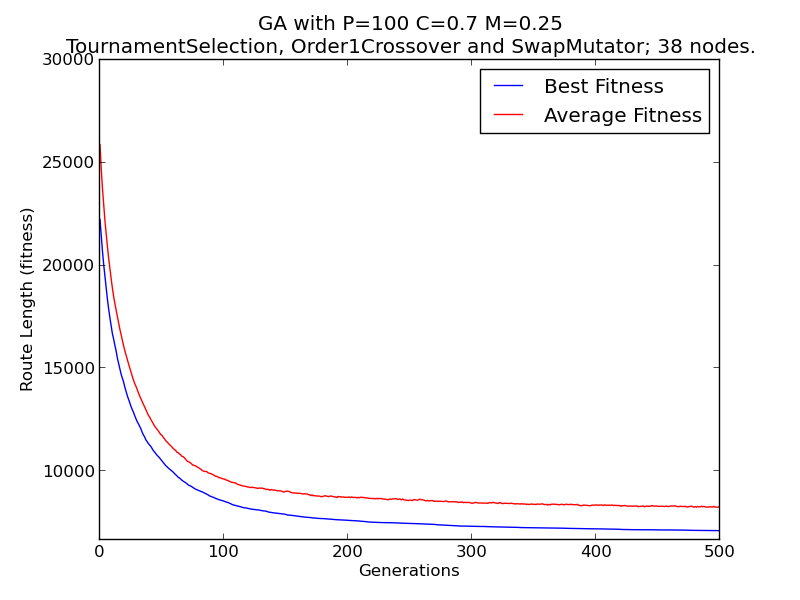
\includegraphics[width=\textwidth]{img/results/order1crossover/swapmutator/n38p100c07m025}
\caption{Swap Mutation Operator}
\end{subfigure}
~
\begin{subfigure}[b]{0.67\textwidth}
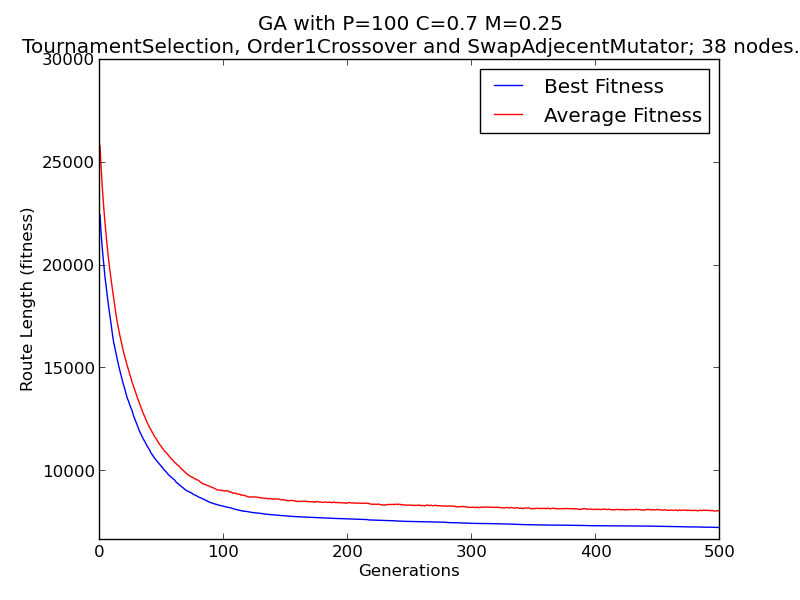
\includegraphics[width=\textwidth]{img/results/order1crossover/swapadjecentmutator/n38p100c07m025}
\caption{Swap Adjacent Mutation Operator}
\end{subfigure}
\caption{Results on different mutation operators on a data set with 38 nodes.
         All used a population of 100, crossover rate of 0.7, mutation rate of
         0.25 and with the order crossover operator}
\label{fig:mutation-results}
\end{figure}


\subsection{Applying the GA to larger problems}

Another important application of a GA is the ability to apply it to larger data
sets. Due to time limitations the number of runs the results are averaged over
has been reduced to 25, but the number of generations has been increased to 
1000 to allow the GA more opportunity to reach optimal values. The problem used
had a total of 194 nodes.

To further compare the crossover schemes from earlier, the time taken to
execute was also recorded using the GNU Tools \texttt{time} command. These
results are shown in table~\ref{tab:time-results} and the graphs are shown in
figure~\ref{fig:time-graph-results}.

\begin{table}[h]
\centering
\begin{tabular}{|c|c|c|c|c|} \hline
\textbf{Crossover Operator}	& \textbf{User}	&\textbf{System}&\textbf{CPU}	& \textbf{Total} \\ \hline
Cycle Crossover			& 1150.65s	& 0.22s		& 99\%		& 19:12.02 \\ \hline
Order Crossover Operator	& 1665.10s	& 0.12s		& 99\%		& 27:46.47 \\ \hline
M-Crossover Operator		& 12998.65s	& 1.00s		& 99\%		& 3:36:54.00\\ \hline
\end{tabular}
\caption{Results of the \texttt{time} command for the different crossover
         operators on a GA with a population of 100, crossover rate of 0.7,
         mutation rate of 0.1 and with the swap mutation operator.}
\label{tab:time-results}
\end{table}

It is interesting to see that cycle crossover is somewhat faster for faster for
larger problems, but the difference in best solution is so big enough that the
extra processing time seems worth it.

The amount of time it takes for the m-crossover operator take to complete is so
slow that it doesn't seem worth it. However, looking at the graphs, a good
results was gained in less than 200 generations, and the rest of the time was
spent slowly optimising the solution.

\begin{figure}[h]
\centering
\begin{subfigure}[b]{0.67\textwidth}
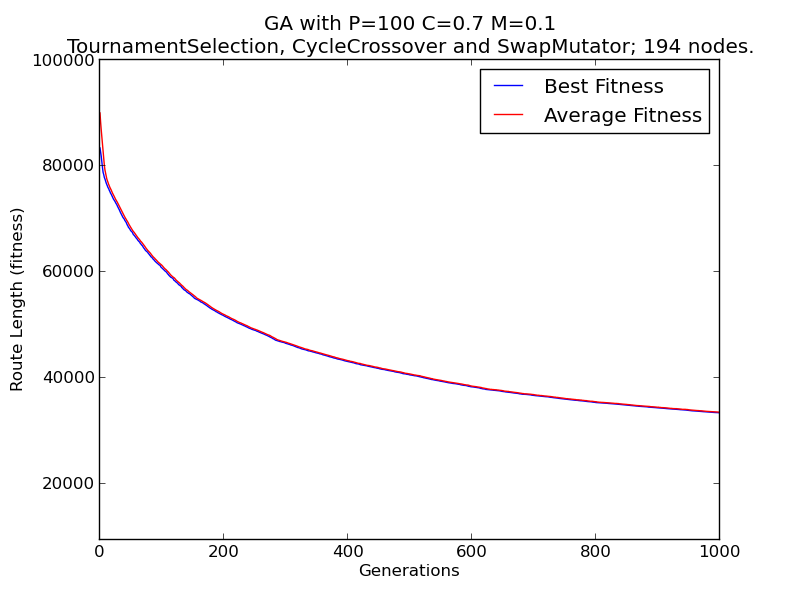
\includegraphics[width=\textwidth]{img/results/cyclecrossover/swapmutator/n194p100c07m01}
\caption{Cycle Crossover}
\end{subfigure}

\begin{subfigure}[b]{0.67\textwidth}
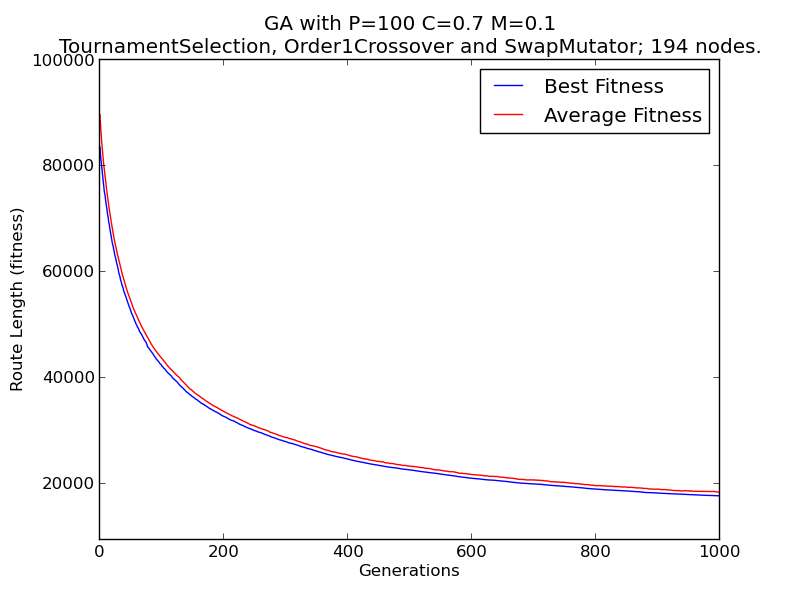
\includegraphics[width=\textwidth]{img/results/order1crossover/swapmutator/n194p100c07m01}
\caption{Order Crossover Operator}
\end{subfigure}

\begin{subfigure}[b]{0.67\textwidth}
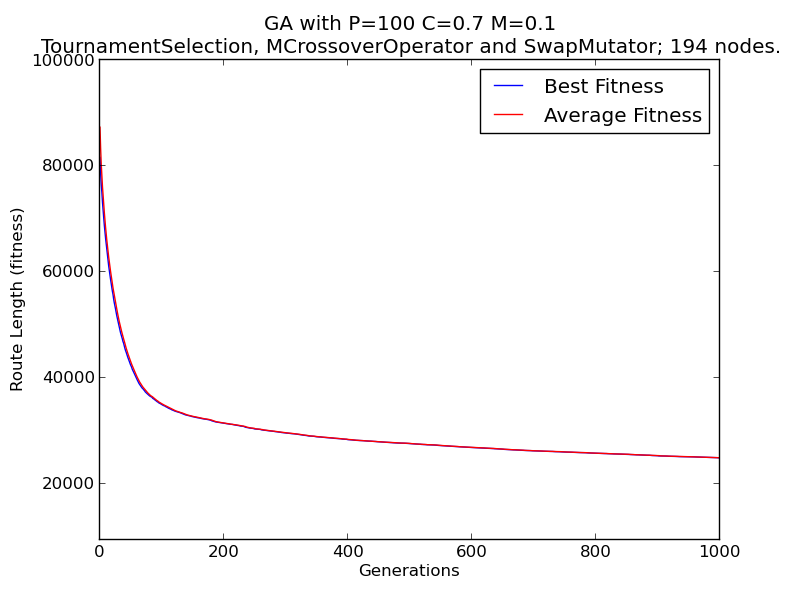
\includegraphics[width=\textwidth]{img/results/mcrossoveroperator/swapmutator/n194p100c07m01}
\caption{M-Crossover Operator}
\end{subfigure}

\caption{Results on different crossover operators on a data set with 194 nodes.
         All used a population of 100, crossover rate of 0.7, mutation rate of 
         0.1 and the swap mutator}
\label{fig:time-graph-results}
\end{figure}


\subsubsection{Getting Early Results}

All the m-crossover operator performs well in the early stage of the GA it
seems fair to compare how each crossover operator performs with a limited 
number of generation. A smaller problem with 29 nodes was chosen. The GAs were
given 50 generations to run and were averaged over 100 runs.

Figure~\ref{fig:early-cutoff-results} shows the experimental results.

Again, the m-crossover operator optimises the solution in very few generations,
but the order crossover operator still manages to compete well with it. If the
generations had of been limited to 15, the m-crossover operator would have been
a useful technique and, certainly for larger data sets, it may be very useful
for the use of gaining a very quick approximate.

\begin{figure}[h]
\centering
\begin{subfigure}[b]{0.67\textwidth}
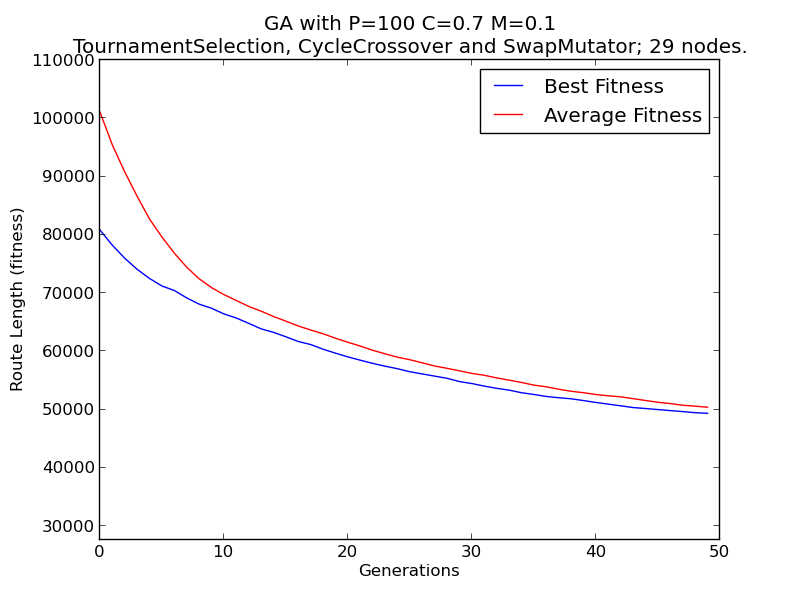
\includegraphics[width=\textwidth]{img/results/cyclecrossover/swapmutator/n29p100c07m01}
\caption{Cycle Crossover}
\end{subfigure}

\begin{subfigure}[b]{0.67\textwidth}
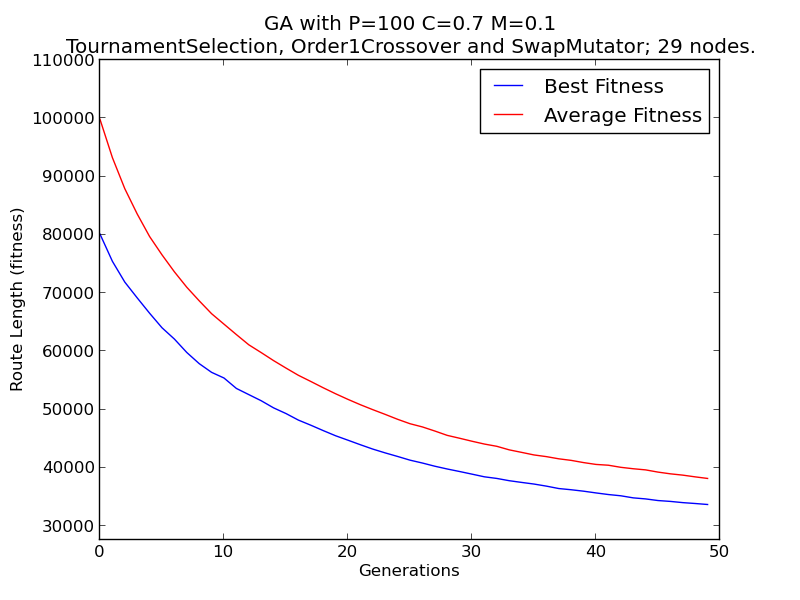
\includegraphics[width=\textwidth]{img/results/order1crossover/swapmutator/n29p100c07m01}
\caption{Order Crossover Operator}
\end{subfigure}

\begin{subfigure}[b]{0.67\textwidth}
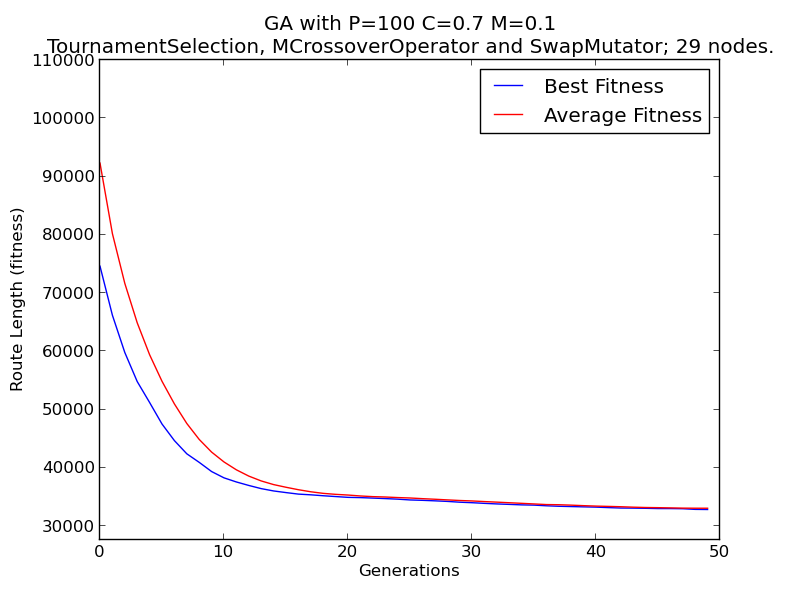
\includegraphics[width=\textwidth]{img/results/mcrossoveroperator/swapmutator/n29p100c07m01}
\caption{M-Crossover Operator}
\end{subfigure}
\caption{Results on different crossover operators on a data set with 29 nodes.
         All used a population of 100, crossover rate of 0.7, mutation rate of
         0.1, with the swap mutation operator. This was cut off after only a
         short number of generations}
\label{fig:early-cutoff-results}

\end{figure}


\newpage
\section{Conclusions}

The order crossover operator is one of the simplest and best crossover 
operators for ordered chromosomes which is computationally cheap to use. Though
it does have some flaws, particularly seeming never to truly converge, its
performance from the above results are fairly conclusive that it can reach a
solution very close to the optimal given enough time.

Unfortunately, the m-crossover operator did not perform as well as expected and
the time complexity of it means that it might not be applicable to large
problems. This does not agree with the research which suggested
it\cite{Mudaliar2013Unraveling} as order crossover operators performed worse in
their experiments. Because they did not take into account the exact tour length
and only used a simplified approach, it would seem that they did not get
accurate results. 

Their results do agree that the m-crossover operator performs well in early 
generation, but slows quickly. However, with some optimisation and 
multi-threading, it may be fast enough to get a reasonable solution to a 
problem in a short period of time, where any other crossover operator would
require more generations to come to a good solution.

It may be the case that the m-crossover operator might benefit from having the
same process of selection performed upon it as the GA would, rather than just
selecting the best two offspring. Further research should follow to investigate
and evaluate this topic.

Due to time constraints, selection schemes were not investigated and tournament
selection was used for all experimental results. A case could be made that
tournament selection was not the best selection scheme for some of the
researched fields. However, the authors previous work into the field would 
suggest that tournament selection is very good for most applications. It might
be worth implementing a roulette wheel selection scheme at a later date to
properly verify the results.

The method used to perform throw away was not the best, choosing a proportion
based on the crossover rate seems to have skewed the results for the crossover
rate experiments, elite preservation might have been a better strategy as the
ratio of offspring to parents would have been kept stable and would have made
the results more comparable.

\bibliographystyle{plain}
\bibliography{citations}

\end{document}
